\documentclass[]{book}
\usepackage{lmodern}
\usepackage{amssymb,amsmath}
\usepackage{ifxetex,ifluatex}
\usepackage{fixltx2e} % provides \textsubscript
\ifnum 0\ifxetex 1\fi\ifluatex 1\fi=0 % if pdftex
  \usepackage[T1]{fontenc}
  \usepackage[utf8]{inputenc}
\else % if luatex or xelatex
  \ifxetex
    \usepackage{mathspec}
  \else
    \usepackage{fontspec}
  \fi
  \defaultfontfeatures{Ligatures=TeX,Scale=MatchLowercase}
\fi
% use upquote if available, for straight quotes in verbatim environments
\IfFileExists{upquote.sty}{\usepackage{upquote}}{}
% use microtype if available
\IfFileExists{microtype.sty}{%
\usepackage{microtype}
\UseMicrotypeSet[protrusion]{basicmath} % disable protrusion for tt fonts
}{}
\usepackage[margin=1in]{geometry}
\usepackage{hyperref}
\hypersetup{unicode=true,
            pdftitle={Math (P)refresher for Political Scientists},
            pdfauthor={Shiro Kuriwaki and Yon Soo Park},
            pdfborder={0 0 0},
            breaklinks=true}
\urlstyle{same}  % don't use monospace font for urls
\usepackage{natbib}
\bibliographystyle{apalike}
\usepackage{color}
\usepackage{fancyvrb}
\newcommand{\VerbBar}{|}
\newcommand{\VERB}{\Verb[commandchars=\\\{\}]}
\DefineVerbatimEnvironment{Highlighting}{Verbatim}{commandchars=\\\{\}}
% Add ',fontsize=\small' for more characters per line
\usepackage{framed}
\definecolor{shadecolor}{RGB}{248,248,248}
\newenvironment{Shaded}{\begin{snugshade}}{\end{snugshade}}
\newcommand{\KeywordTok}[1]{\textcolor[rgb]{0.13,0.29,0.53}{\textbf{#1}}}
\newcommand{\DataTypeTok}[1]{\textcolor[rgb]{0.13,0.29,0.53}{#1}}
\newcommand{\DecValTok}[1]{\textcolor[rgb]{0.00,0.00,0.81}{#1}}
\newcommand{\BaseNTok}[1]{\textcolor[rgb]{0.00,0.00,0.81}{#1}}
\newcommand{\FloatTok}[1]{\textcolor[rgb]{0.00,0.00,0.81}{#1}}
\newcommand{\ConstantTok}[1]{\textcolor[rgb]{0.00,0.00,0.00}{#1}}
\newcommand{\CharTok}[1]{\textcolor[rgb]{0.31,0.60,0.02}{#1}}
\newcommand{\SpecialCharTok}[1]{\textcolor[rgb]{0.00,0.00,0.00}{#1}}
\newcommand{\StringTok}[1]{\textcolor[rgb]{0.31,0.60,0.02}{#1}}
\newcommand{\VerbatimStringTok}[1]{\textcolor[rgb]{0.31,0.60,0.02}{#1}}
\newcommand{\SpecialStringTok}[1]{\textcolor[rgb]{0.31,0.60,0.02}{#1}}
\newcommand{\ImportTok}[1]{#1}
\newcommand{\CommentTok}[1]{\textcolor[rgb]{0.56,0.35,0.01}{\textit{#1}}}
\newcommand{\DocumentationTok}[1]{\textcolor[rgb]{0.56,0.35,0.01}{\textbf{\textit{#1}}}}
\newcommand{\AnnotationTok}[1]{\textcolor[rgb]{0.56,0.35,0.01}{\textbf{\textit{#1}}}}
\newcommand{\CommentVarTok}[1]{\textcolor[rgb]{0.56,0.35,0.01}{\textbf{\textit{#1}}}}
\newcommand{\OtherTok}[1]{\textcolor[rgb]{0.56,0.35,0.01}{#1}}
\newcommand{\FunctionTok}[1]{\textcolor[rgb]{0.00,0.00,0.00}{#1}}
\newcommand{\VariableTok}[1]{\textcolor[rgb]{0.00,0.00,0.00}{#1}}
\newcommand{\ControlFlowTok}[1]{\textcolor[rgb]{0.13,0.29,0.53}{\textbf{#1}}}
\newcommand{\OperatorTok}[1]{\textcolor[rgb]{0.81,0.36,0.00}{\textbf{#1}}}
\newcommand{\BuiltInTok}[1]{#1}
\newcommand{\ExtensionTok}[1]{#1}
\newcommand{\PreprocessorTok}[1]{\textcolor[rgb]{0.56,0.35,0.01}{\textit{#1}}}
\newcommand{\AttributeTok}[1]{\textcolor[rgb]{0.77,0.63,0.00}{#1}}
\newcommand{\RegionMarkerTok}[1]{#1}
\newcommand{\InformationTok}[1]{\textcolor[rgb]{0.56,0.35,0.01}{\textbf{\textit{#1}}}}
\newcommand{\WarningTok}[1]{\textcolor[rgb]{0.56,0.35,0.01}{\textbf{\textit{#1}}}}
\newcommand{\AlertTok}[1]{\textcolor[rgb]{0.94,0.16,0.16}{#1}}
\newcommand{\ErrorTok}[1]{\textcolor[rgb]{0.64,0.00,0.00}{\textbf{#1}}}
\newcommand{\NormalTok}[1]{#1}
\usepackage{longtable,booktabs}
\usepackage{graphicx,grffile}
\makeatletter
\def\maxwidth{\ifdim\Gin@nat@width>\linewidth\linewidth\else\Gin@nat@width\fi}
\def\maxheight{\ifdim\Gin@nat@height>\textheight\textheight\else\Gin@nat@height\fi}
\makeatother
% Scale images if necessary, so that they will not overflow the page
% margins by default, and it is still possible to overwrite the defaults
% using explicit options in \includegraphics[width, height, ...]{}
\setkeys{Gin}{width=\maxwidth,height=\maxheight,keepaspectratio}
\IfFileExists{parskip.sty}{%
\usepackage{parskip}
}{% else
\setlength{\parindent}{0pt}
\setlength{\parskip}{6pt plus 2pt minus 1pt}
}
\setlength{\emergencystretch}{3em}  % prevent overfull lines
\providecommand{\tightlist}{%
  \setlength{\itemsep}{0pt}\setlength{\parskip}{0pt}}
\setcounter{secnumdepth}{5}
% Redefines (sub)paragraphs to behave more like sections
\ifx\paragraph\undefined\else
\let\oldparagraph\paragraph
\renewcommand{\paragraph}[1]{\oldparagraph{#1}\mbox{}}
\fi
\ifx\subparagraph\undefined\else
\let\oldsubparagraph\subparagraph
\renewcommand{\subparagraph}[1]{\oldsubparagraph{#1}\mbox{}}
\fi

%%% Use protect on footnotes to avoid problems with footnotes in titles
\let\rmarkdownfootnote\footnote%
\def\footnote{\protect\rmarkdownfootnote}

%%% Change title format to be more compact
\usepackage{titling}

% Create subtitle command for use in maketitle
\newcommand{\subtitle}[1]{
  \posttitle{
    \begin{center}\large#1\end{center}
    }
}

\setlength{\droptitle}{-2em}
  \title{Math (P)refresher for Political Scientists}
  \pretitle{\vspace{\droptitle}\centering\huge}
  \posttitle{\par}
  \author{Shiro Kuriwaki and Yon Soo Park}
  \preauthor{\centering\large\emph}
  \postauthor{\par}
  \predate{\centering\large\emph}
  \postdate{\par}
  \date{2018-06-17}

\usepackage{booktabs}

\usepackage{epsfig}
\usepackage{epstopdf}
\usepackage{rotate}
\usepackage{graphicx}
\usepackage{hyperref}
\usepackage{alphalph}
\usepackage{caption}
\usepackage[hang,flushmargin]{footmisc}
\usepackage{framed}
\usepackage{xcolor}
\usepackage{verbatim} 

\setcounter{MaxMatrixCols}{20}
\newcommand{\Var}{\mathrm{Var}}
\newcommand{\SD}{\mathrm{SD}}
\newcommand{\Cov}{\mathrm{Cov}}
\newcommand{\fx}{f({\bf x})}
\newcommand\R{{\textsf R~}}
\newcommand\Rst{\textsf{RStudio}}

\oddsidemargin=0in
\evensidemargin=0in
\textwidth=6.5in
\topmargin=0in
\headsep=.25in
\headheight=.25in
\textheight=9.25in
\topskip=0in
\voffset=-0.5in
\epsfxsize=1in

\usepackage{amsthm}
\newtheorem{theorem}{Theorem}[chapter]
\newtheorem{lemma}{Lemma}[chapter]
\theoremstyle{definition}
\newtheorem{definition}{Definition}[chapter]
\newtheorem{corollary}{Corollary}[chapter]
\newtheorem{proposition}{Proposition}[chapter]
\theoremstyle{definition}
\newtheorem{example}{Example}[chapter]
\theoremstyle{definition}
\newtheorem{exercise}{Exercise}[chapter]
\theoremstyle{remark}
\newtheorem*{remark}{Remark}
\newtheorem*{solution}{Solution}
\begin{document}
\maketitle

{
\setcounter{tocdepth}{1}
\tableofcontents
}
\chapter{Welcome}\label{welcome}

The documents in this booklet are the product of generations of Math
(P)refresher Instructors: Curt Signorino 1996-1997; Ken Scheve
1997-1998; Eric Dickson 1998-2000; Orit Kedar 1999; James Fowler
2000-2001; Kosuke Imai 2001-2002; Jacob Kline 2002; Dan Epstein 2003;
Ben Ansell 2003-2004; Ryan Moore 2004-2005; Mike Kellermann 2005-2006;
Ellie Powell 2006-2007; Jen Katkin 2007-2008; Patrick Lam 2008-2009;
Viridiana Rios 2009-2010; Jennifer Pan 2010-2011; Konstantin Kashin
2011-2012; Sol'\{e\} Prillaman 2013; Stephen Pettigrew 2013-2014; Anton
Strezhnev 2014-2015; Mayya Komisarchik 2015-2016; Connor Jerzak
2016-2017; Shiro Kuriwaki 2017-2018; Yon Soo Park 2018-.

\chapter{Functions and Notation}\label{functions-and-notation}

\textbf{Topics} Dimensionality; Interval Notation for \({\bf R}^1\);
Neighborhoods: Intervals, Disks, and Balls; Introduction to Functions;
Domain and Range; Some General Types of Functions; \(\log\), \(\ln\),
and \(\exp\); Other Useful Functions; Graphing Functions; Solving for
Variables; Finding Roots; Limit of a Function; Continuity; Sets, Sets,
and More Sets.

Much of the material and examples for this lecture are taken from Simon
\& Blume (1994) \emph{Mathematics for Economists}, Boyce \& Diprima
(1988) \emph{Calculus}, and Protter \& Morrey (1991)
\emph{A First Course in Real Analysis}

\section{Dimensionality}\label{dimensionality}

\({\bf R}^1\) is the set of all real numbers extending from \(-\infty\)
to \(+\infty\) --- i.e., the real number line. \({\bf R}^n\) is an
\(n\)-dimensional space (often referred to as Euclidean space), where
each of the \(n\) axes extends from \(-\infty\) to \(+\infty\).

\begin{itemize}
\tightlist
\item
  \({\bf R}^1\) is a one dimensional line.
\item
  \({\bf R}^2\) is a two dimensional plane.
\item
  \({\bf R}^3\) is a three dimensional space.
\item
  \({\bf R}^4\) could be 3-D plus time (or temperature, etc).
\end{itemize}

Points in \({\bf R}^n\) are ordered \(n\)-tuples, where each element of
the \(n\)-tuple represents the coordinate along that dimension.

\begin{itemize}
\tightlist
\item
  \({\bf R}^1\): (3)
\item
  \({\bf R}^2\): (-15, 5)
\item
  \({\bf R}^3\): (86, 4, 0)
\end{itemize}

\section{\texorpdfstring{Interval Notation for
\({\bf R}^1\)}{Interval Notation for \{\textbackslash{}bf R\}\^{}1}}\label{interval-notation-for-bf-r1}

Open interval: \[(a,b)\equiv \{ x\in{\bf R}^1: a<x<b\}\]

\(x\) is a one-dimensional element in which x is greater than a and less
than b

Closed interval: \[[a,b]\equiv \{ x\in{\bf R}^1: a\le x \le b\}\]

\(x\) is a one-dimensional element in which x is greater or equal to
than a and less than or equal to b

Half open, half closed: \[(a,b]\equiv \{ x\in{\bf R}^1: a<x\le b\}\]

\(x\) is a one-dimensional element in which x is greater than a and less
than or equal to b

\section{Neighborhoods: Intervals, Disks, and
Balls}\label{neighborhoods-intervals-disks-and-balls}

In many areas of math, we need a formal construct for what it means to
be ``near'' a point \(\bf c\) in \({\bf R}^n\). This is generally called
the \textbf{neighborhood} of \(\bf c\). It's represented by an open
interval, disk, or ball, depending on whether \({\bf R}^n\) is of one,
two, or more dimensions, respectively.

Given the point \(c\), these are defined as

\begin{itemize}
\tightlist
\item
  \(\epsilon\)-interval in \({\bf R}^1\): \(\{x : |x-c|<\epsilon \}\).
  \(x\) is in the neighborhood of \{\bf c\} if it is in the open
  interval \((c-\epsilon,c+\epsilon)\).
\item
  \(\epsilon\)-disk in \({\bf R}^2\): \(\{x : || x-c ||<\epsilon\}\).
  \(x\) is in the neighborhood of \{\bf c\} if it is inside the circle
  or disc with center \(\bf c\) and radius \(\epsilon\).
\item
  \(\epsilon\)-ball in \({\bf R}^n\): \(\{x : || x-c ||<\epsilon\}\).
  \(x\) is in the neighborhood of \{\bf c\} if it is inside the sphere
  or ball with center \(\bf c\) and radius \(\epsilon\).
\end{itemize}

\section{Introduction to Functions}\label{introduction-to-functions}

A \textbf{function} (in \({\bf R}^1\)) is a mapping, or transformation,
that relates members of one set to members of another set. For instance,
if you have two sets: set \(A\) and set \(B\), a function from \(A\) to
\(B\) maps every value \(a\) in set \(A\) such that \(f(a) \in B\).
Functions can be ``many-to-one'', where many values or combinations of
values from set \(A\) produce a single output in set \(B\), or they can
be ``one-to-one'', where each value in set \(A\) corresponds to a single
value in set \(B\).

Examples: Mapping notation

\begin{itemize}
\tightlist
\item
  Function of one variable: \(f:{\bf R}^1\to{\bf R}^1\)\textbackslash{}
  \(f(x)=x+1\). For each \(x\) in \({\bf R}^1\), \(f(x)\) assigns the
  number \(x+1\).
\item
  Function of two variables: \(f: {\bf R}^2\to{\bf R}^1\).
  \(f(x,y)=x^2+y^2\). For each ordered pair \((x,y)\) in \({\bf R}^2\),
  \(f(x,y)\) assigns the number \(x^2+y^2\).
\end{itemize}

We often use variable \(x\) as input and another \(y\) as output, e.g.
\(y=x+1\)

\section{Domain and Range/Image}\label{domain-and-rangeimage}

Some functions are defined only on proper subsets of \({\bf R}^n\).

\begin{itemize}
\tightlist
\item
  \textbf{Domain}: the set of numbers in \(X\) at which \(f(x)\) is
  defined.
\item
  \textbf{Range}: elements of \(Y\) assigned by \(f(x)\) to elements of
  \(X\), or \[f(X)=\{ y : y=f(x), x\in X\}\] Most often used when
  talking about a function \(f:{\bf R}^1\to{\bf R}^1\).
\item
  \textbf{Image}: same as range, but more often used when talking about
  a function \(f:{\bf R}^n\to{\bf R}^1\).
\end{itemize}

\section{Some General Types of
Functions}\label{some-general-types-of-functions}

\textbf{Monomials}: \(f(x)=a x^k\)\textbackslash{} \(a\) is the
coefficient. \(k\) is the degree.\textbackslash{} Examples: \(y=x^2\),
\(y=-\frac{1}{2}x^3\)

\textbf{Polynomials}: sum of monomials. Examples:
\(y=-\frac{1}{2}x^3+x^2\), \(y=3x+5\)

The degree of a polynomial is the highest degree of its monomial terms.
Also, it's often a good idea to write polynomials with terms in
decreasing degree.

\textbf{Rational Functions}: ratio of two polynomials.

Examples: \(y=\frac{x}{2}\), \(y=\frac{x^2+1}{x^2-2x+1}\)

\textbf{Exponential Functions}: Example: \(y=2^x\)

\textbf{Trigonometric Functions}: Examples: \(y=\cos(x)\),
\(y=3\sin(4x)\)

\begin{comment}
    \parbox[c]{4.75in}{{\bf Linear}: polynomial of degree 1.\\
        Example: $y=m x + b$, where $m$ is the slope and $b$ is the $y$-intercept.}\epsfxsize=1in \parbox{1in}{\, {\includegraphics[width=.9in, angle = 270]{linear.eps}}}
    
    \item \parbox[c]{4.75in}{{\bf Nonlinear}: anything that isn't constant or polynomial of degree 1.\\
        Examples:  $y=x^2+2x+1$, $y=\sin(x)$, $y=\ln(x)$, $y=e^x$}
        \parbox{1in}{\,  {\includegraphics[width=.9in, angle = 270]{nonlin.eps}}}
\end{comment}

\section{\texorpdfstring{\(\log\), \(\ln\), and
\(\exp\)}{\textbackslash{}log, \textbackslash{}ln, and \textbackslash{}exp}}\label{log-ln-and-exp}

\textbf{Relationship of logarithmic and exponential functions}:
\[y=\log_a(x) \iff a^y=x\]

The log function can be thought of as an inverse for exponential
functions. \(a\) is referred to as the ``base'' of the logarithm.

\textbf{Common Bases}: The two most common logarithms are base 10 and
base \(e\).

\begin{enumerate}
\def\labelenumi{\arabic{enumi}.}
\tightlist
\item
  Base 10: \(\quad y=\log_{10}(x) \iff 10^y=x\). The base 10 logarithm
  is often simply written as ``\(\log(x)\)'' with no base denoted.
\item
  Base \(e\): \(\quad y=\log_e(x) \iff e^y=x\). The base \(e\) logarithm
  is referred to as the ``natural'' logarithm and is written as
  ``\(\ln(x)\)``.
\end{enumerate}

\begin{comment}
            {\includegraphics[width=1in, angle = 270]{ln.eps}} \,  {\includegraphics[width=1in, angle = 270]{exp.eps}}
            \end{comment}

\textbf{Properties of exponential functions:}

\begin{itemize}
\tightlist
\item
  \(a^x a^y = a^{x+y}\)
\item
  \(a^{-x} = 1/a^x\)
\item
  \(a^x/a^y = a^{x-y}\)
\item
  \((a^x)^y = a^{x y}\)
\item
  \(a^0 = 1\)
\end{itemize}

\textbf{Properties of logarithmic functions} (any base):

Generally, when statisticians or social scientists write \(\log(x)\)
they mean \(\log_e(x)\). In other words:
\(\log_e(x) \equiv \ln(x) \equiv \log(x)\)

\[\log_a(a^x)=x\] and \[a^{\log_a(x)}=x\]

\begin{itemize}
\tightlist
\item
  \(\log(x y)=\log(x)+\log(y)\)
\item
  \(\log(x^y)=y\log(x)\)
\item
  \(\log(1/x)=\log(x^{-1})=-\log(x)\)
\item
  \(\log(x/y)=\log(x\cdot y^{-1})=\log(x)+\log(y^{-1})=\log(x)-\log(y)\)
\item
  \(\log(1)=\log(e^0)=0\)
\end{itemize}

\textbf{Change of Base Formula}: Use the change of base formula to
switch bases as necessary: \[\log_b(x) = \frac{\log_a(x)}{\log_a(b)}\]

Example: \[\log_{10}(x) = \frac{\ln(x)}{\ln(10)}\]

\begin{itemize}
\item $\log_{10}(\sqrt{10})=\log_{10}(10^{1/2}) = $
\item $\log_{10}(1)=\log_{10}(10^{0}) = $
\item $\log_{10}(10)=\log_{10}(10^{1}) = $
\item $\log_{10}(100)=\log_{10}(10^{2}) = $
\item $\ln(1)=\ln(e^{0}) = $
\item $\ln(e)=\ln(e^{1}) = $
\end{itemize}

\section{Other Useful Functions}\label{other-useful-functions}

\textbf{Factorials!:}

\[x! = x\cdot (x-1) \cdot (x-2) \cdots (1)\]

\textbf{Modulo:} Tells you the remainder when you divide one number by
another. Can be extremely useful for programming: \texttt{x mod y} or
\texttt{x \% y}

\begin{itemize}
\tightlist
\item
  \(17 \mod 3 = 2\)
\item
  \(100 \ \% \ 30 = 10\)
\end{itemize}

\textbf{Summation:}

\[\sum\limits_{i=1}^n x_i = x_1+x_2+x_3+\cdots+x_n\]

\begin{itemize}
\item $\sum\limits_{i=1}^n c x_i = c \sum\limits_{i=1}^n x_i $
\item $\sum\limits_{i=1}^n (x_i + y_i) =  \sum\limits_{i=1}^n x_i + \sum\limits_{i=1}^n y_i $
\item $\sum\limits_{i=1}^n c = n c $
\end{itemize}

\textbf{Product:}

\[\prod\limits_{i=1}^n x_i = x_1 x_2 x_3 \cdots x_n\]

Properties:

\begin{itemize}
\item $\prod\limits_{i=1}^n c x_i = c^n \prod\limits_{i=1}^n x_i $
\item $\prod\limits_{i=1}^n (x_i + y_i) =$ a total mess
\item $\prod\limits_{i=1}^n c = c^n $
\end{itemize}

You can use logs to go between sum and product notation. This will be
particularly important when you're learning maximum likelihood
estimation.

\begin{eqnarray*}
            \log \bigg(\prod\limits_{i=1}^n x_i \bigg) &=& \log(x_1 \cdot x_2 \cdot x_3 \cdots \cdot x_n)\\
            &=& \log(x_1) + \log(x_2) + \log(x_3) + \cdots + \log(x_n)\\
            &=& \sum\limits_{i=1}^n \log (x_i)
\end{eqnarray*}

Therefore, you can see that the log of a product is equal to the sum of
the logs. We can write this more generally by adding in a constant,
\(c\):

\begin{eqnarray*}
            \log \bigg(\prod\limits_{i=1}^n c x_i\bigg) &=& \log(cx_1 \cdot cx_2 \cdots cx_n)\\
            &=& \log(c^n \cdot x_1 \cdot x_2 \cdots x_n)\\
            &=& \log(c^n) + \log(x_1) + \log(x_2) + \cdots + \log(x_n)\\\\
            &=& n \log(c) +  \sum\limits_{i=1}^n \log (x_i)\\
\end{eqnarray*}

\section{Graphing Functions}\label{graphing-functions}

What can a graph tell you about a function?

\begin{itemize}
\tightlist
\item
  Is the function increasing or decreasing? Over what part of the
  domain?
\item
  How ``fast" does it increase or decrease?
\item
  Are there global or local maxima and minima? Where?
\item
  Are there inflection points?
\item
  Is the function continuous?
\item
  Is the function differentiable?
\item
  Does the function tend to some limit?
\item
  Other questions related to the substance of the problem at hand.
\end{itemize}

\section{Solving for Variables and Finding
Inverses}\label{solving-for-variables-and-finding-inverses}

Sometimes we're given a function \(y=f(x)\) and we want to find how
\(x\) varies as a function of \(y\). If \(f\) is a one-to-one mapping,
then it has an inverse.

Use algebra to move \(x\) to the left hand side (LHS) of the equation
and so that the right hand side (RHS) is only a function of
\(y\).\textbackslash{}

Examples: (we want to solve for \(x\))

\[y=3x+2 \quad\Longrightarrow\quad -3x=2-y \quad\Longrightarrow\quad 3x=y-2 \quad\Longrightarrow\quad x=\frac{1}{3}(y-2)\]
\[y=3x-4z+2 \quad \Longrightarrow\quad y+4z-2=3x \quad\Longrightarrow\quad x=\frac{1}{3}(y+4z-2)\]
\[y=e^x+4 \quad\Longrightarrow\quad y-4=e^x \quad\Longrightarrow\quad \ln(y-4)=\ln(e^x)\quad\Longrightarrow\quad x=\ln(y-4)\]

Sometimes (often?) the inverse does not exist. For example, we're given
the function \(y=x^2\) (a parabola). Solving for \(x\), we get
\(x=\pm\sqrt{y}\). For each value of \(y\), there are two values of
\(x\).

\section{Finding the Roots or Zeroes of a
Function}\label{finding-the-roots-or-zeroes-of-a-function}

Solving for variables is especially important when we want to find the
\textbf{roots} of an equation: those values of variables that cause an
equation to equal zero. Especially important in finding equilibria and
in doing maximum likelihood estimation.

Procedure: Given \(y=f(x)\), set \(f(x)=0\). Solve for \(x\).

Multiple Roots:
\[f(x)=x^2 - 9 \quad\Longrightarrow\quad 0=x^2 - 9 \quad\Longrightarrow\quad 9=x^2 \quad\Longrightarrow\quad \pm \sqrt{9}=\sqrt{x^2} \quad\Longrightarrow\quad \pm 3=x\]

\textbf{Quadratic Formula:} For quadratic equations \(ax^2+bx+c=0\), use
the quadratic formula: \[x=\frac{-b\pm\sqrt{b^2-4ac}}{2a}\]

Examples:

\begin{enumerate}
        \item $f(x)=3x+2$ \\
        % $\quad\Longrightarrow\quad 3x+2=0 
        % \quad\Longrightarrow\quad x=-\frac{2}{3}$\\
        \item $f(x)=e^{-x}-10$ \\
        %$\quad\Longrightarrow\quad e^{-x}-10=0 
        %\quad\Longrightarrow\quad e^{-x}=10 \quad\Longrightarrow\quad 
        %x=-\ln(10)$\\
        \item $f(x)=x^2+3x-4=0$  \\
        %$\quad\Longrightarrow\quad x=\{1,-4\}$\\
\end{enumerate}

\section{The Limit of a Function}\label{the-limit-of-a-function}

We're often interested in determining if a function \(f\) approaches
some number \(L\) as its independent variable \(x\) moves to some number
\(c\) (usually 0 or \(\pm\infty\)). If it does, we say that the limit of
\(f(x)\), as \(x\) approaches \(c\), is \(L\):
\(\lim\limits_{x \to c} f(x)=L\).

For a limit \(L\) to exist, the function \(f(x)\) must approach \(L\)
from both the left and right.

\textbf{Limit of a function}. Let \(f(x)\) be defined at each point in
some open interval containing the point \(c\). Then \(L\) equals
\(\lim\limits_{x \to c} f(x)\) if for any (small positive) number
\(\epsilon\), there exists a corresponding number \(\delta>0\) such that
if \(0<|x-c|<\delta\), then \(|f(x)-L|<\epsilon\).

Note: f(x) does not necessarily have to be defined at \(c\) for
\(\lim\limits_{x \to c}\) to exist.

\textbf{Uniqueness}: \(\lim\limits_{x \to c} f(x)=L\) and
\(\lim\limits_{x \to c} f(x)=M \Longrightarrow L=M\)

Properties: Let \(f\) and \(g\) be functions with
\(\lim\limits_{x \to c} f(x)=A\) and \(\lim\limits_{x \to c} g(x)=B\).

\begin{itemize}
\tightlist
\item
  \(\lim\limits_{x \to c}[f(x)+g(x)]=\lim\limits_{x \to c} f(x)+ \lim\limits_{x \to c} g(x)\)
\item
  \(\lim\limits_{x \to c} \alpha f(x) = \alpha \lim\limits_{x \to c} f(x)\)
\item
  \(\lim\limits_{x \to c} f(x) g(x) = [\lim\limits_{x \to c} f(x)][\lim\limits_{x \to c} g(x)]\)
\item
  \(\lim\limits_{x \to c} \frac{f(x)}{g(x)} = \frac{\lim\limits_{x \to c} f(x)}{\lim\limits_{x \to c} g(x)}\),
  provided \(\lim\limits_{x \to c} g(x)\ne 0\).
\end{itemize}

Note: In a couple days we'll talk about L'H\^{}opital's Rule, which uses
simple calculus to help find the limits of functions like this.

Examples:

\begin{align*}
& \lim_{x \to c} k = \\
& \lim_{x \to c} x = \\
& \lim_{x\to 2} (2x-3) =\\
& \lim_{x \to c} x^n = 
\end{align*}

\begin{comment}
%= 2\lim\limits_{x\to 2} x- 3\lim\limits_{x\to 2} 1 = 2\times 2 - 3\times 1 = 1 
%[\lim\limits_{x \to c} x]\cdots[\lim\limits_{x \to c} x] = c\cdots c =c^n 
\end{comment}

\begin{comment}
        \item \parbox[t]{3.75in}{$\lim\limits_{x\to 0} |x| =$} \parbox[t]{1in}{\,{\includegraphics[width=1in, angle = 270]{abs.eps}}} % = 0
        \item \parbox[t]{3.75in}{$\lim\limits_{x\to 0} \left(1+\frac{1}{x^2}\right)=$} \parbox[t]{1in}{\,  {\includegraphics[width=1in, angle = 270]{1p1ovrx2.eps}}} %\infty
\end{comment}

Types of limits:

\begin{enumerate}
\def\labelenumi{\arabic{enumi}.}
\tightlist
\item
  Right-hand limit: The value approached by \(f(x)\) when you move from
  right to left.

  \begin{comment}
      \parbox[t]{2in}{Example:  $\lim\limits_{x\to 0^+} \sqrt{x} = 0$}\parbox[t]{1in}{\,  {\includegraphics[width=1in, angle = 270]{sqrt.eps}}}
      \end{comment}
\item
  Left-hand limit: The value approached by \(f(x)\) when you move from
  left to right.
\item
  Infinity: The value approached by \(f(x)\) as x grows infinitely
  large. Sometimes this may be a number; sometimes it might be
  \(\infty\) or \(-\infty\).
\item
  Negative infinity: The value approached by \(f(x)\) as x grows
  infinitely negative. Sometimes this may be a number; sometimes it
  might be \(\infty\) or \(-\infty\).
\end{enumerate}

\begin{comment}
\parbox[t]{2in}{Example:  $\lim\limits_{x\to \infty} 1/x = \lim\limits_{x\to -\infty} 1/x= 0$}\parbox[t]{1in}{\,  {\includegraphics[width=1in, angle = 270]{1ovrx.eps}}}\\ 
\end{comment}

\section{Continuity}\label{continuity}

\textbf{Continuity}: Suppose that the domain of the function \(f\)
includes an open interval containing the point \(c\). Then \(f\) is
continuous at \(c\) if \(\lim\limits_{x \to c} f(x)\) exists and if
\(\lim\limits_{x \to c} f(x)=f(c)\). Further, \(f\) is continuous on an
open interval \((a,b)\) if it is continuous at each point in the
interval.

Examples: Continuous functions.

\begin{comment}
    \parbox[t]{1.5in}{\hfill$f(x)=\sqrt{x}\quad$}\parbox[t]{1in}{\,  {\includegraphics[width=1in, angle = 270]{sqrt.eps}}}
    \parbox[t]{1.5in}{\hfill$f(x)=e^x\quad$}\parbox[t]{1in}{\,  {\includegraphics[width=1in, angle = 270]{exp.eps}}}
    \item[] Examples: Discontinuous functions.\\
    \parbox[t]{1.5in}{\hfill$f(x)=\mbox{floor}(x)\quad$}\parbox[t]{1in}{\,  {\includegraphics[width=1in, angle = 270]{floor.eps}}}
    \parbox[t]{1.5in}{\hfill$f(x)=1+\frac{1}{x^2}\quad$}\parbox[t]{1in}{\,  {\includegraphics[width=1in, angle = 270]{1p1ovrx2.eps}}}
\end{comment}

Properties:

\begin{enumerate}
\def\labelenumi{\arabic{enumi}.}
\tightlist
\item
  If \(f\) and \(g\) are continuous at point \(c\), then \(f+g\),
  \(f-g\), \(f \cdot g\), \(|f|\), and \(\alpha f\) are continuous at
  point \(c\) also. \(f/g\) is continuous, provided \(g(c)\ne 0\).
\item
  Boundedness: If \(f\) is continuous on the closed bounded interval
  \([a,b]\), then there is a number \(K\) such that \(|f(x)|\le K\) for
  each \(x\) in \([a,b]\).
\item
  Max/Min: If \(f\) is continuous on the closed bounded interval
  \([a,b]\), then \(f\) has a maximum and a minimum on \([a,b]\). They
  may be located at the end points.
\end{enumerate}

\section{Sets}\label{sets}

\textbf{Interior Point}: The point \(\bf x\) is an interior point of the
set \(S\) if \(\bf x\) is in \(S\) and if there is some
\(\epsilon\)-ball around \(\bf x\) that contains only points in \(S\).
The \textbf{interior} of \(S\) is the collection of all interior points
in \(S\). The interior can also be defined as the union of all open sets
in \(S\).

\begin{itemize}
\tightlist
\item
  If the set \(S\) is circular, the interior points are everything
  inside of the circle, but not on the circle's rim.
\item
  Example: The interior of the set \(\{ (x,y) : x^2+y^2\le 4 \}\) is
  \(\{ (x,y) : x^2+y^2< 4 \}\) .
\end{itemize}

\textbf{Boundary Point}: The point \(\bf x\) is a boundary point of the
set \(S\) if every \(\epsilon\)-ball around \(\bf x\) contains both
points that are in \(S\) and points that are outside \(S\). The
\textbf{boundary} is the collection of all boundary points.

\begin{itemize}
\tightlist
\item
  If the set \(S\) is circular, the boundary points are everything on
  the circle's rim.
\item
  Example: The boundary of \(\{ (x,y) : x^2+y^2\le 4 \}\) is
  \(\{ (x,y) : x^2+y^2 = 4 \}\).
\end{itemize}

\textbf{Open}: A set \(S\) is open if for each point \(\bf x\) in \(S\),
there exists an open \(\epsilon\)-ball around \(\bf x\) completely
contained in \(S\).

\begin{itemize}
\tightlist
\item
  If the set \(S\) is circular and open, the points contained within the
  set get infinitely close to the circle's rim, but do not touch it.
\item
  Example: \(\{ (x,y) : x^2+y^2<4 \}\)
\end{itemize}

\textbf{Closed}: A set \(S\) is closed if it contains all of its
boundary points.

\begin{itemize}
\tightlist
\item
  If the set \(S\) is circular and closed, the set contains all points
  within the rim as well as the rim itself.
\item
  Example: \(\{ (x,y) : x^2+y^2\le 4 \}\)
\item
  Note: a set may be neither open nor closed. Example:
  \(\{ (x,y) : 2 < x^2+y^2\le 4 \}\)
\end{itemize}

\textbf{Complement}: The complement of set \(S\) is everything outside
of \(S\).

\begin{itemize}
\tightlist
\item
  If the set \(S\) is circular, the complement of \(S\) is everything
  outside of the circle.
\item
  Example: The complement of \(\{ (x,y) : x^2+y^2\le 4 \}\) is
  \(\{ (x,y) : x^2+y^2 > 4 \}\).
\end{itemize}

\textbf{Closure}: The closure of set \(S\) is the smallest closed set
that contains \(S\).

\begin{itemize}
\tightlist
\item
  Example: The closure of \(\{ (x,y) : x^2+y^2<4 \}\) is
  \(\{ (x,y) : x^2+y^2\le 4 \}\)
\end{itemize}

\textbf{Bounded}: A set \(S\) is bounded if it can be contained within
an \(\epsilon\)-ball.

\begin{itemize}
\tightlist
\item
  Examples: Bounded: any interval that doesn't have \(\infty\) or
  \(-\infty\) as endpoints; any disk in a plane with finite radius.
\item
  Unbounded: the set of integers in \({\bf R}^1\); any ray.
\end{itemize}

\textbf{Compact}: A set is compact if and only if it is both closed and
bounded.

\textbf{Empty}: The empty (or null) set is a unique set that has no
elements, denoted by \{\} or \(\o\).

\begin{itemize}
\tightlist
\item
  Examples: The set of squares with 5 sides; the set of countries south
  of the South Pole.
\item
  The set, \(S\), denoted by \(\{\o\}\) is technically \emph{not} empty.
  That is because this set contains the empty set within it, so \(S\) is
  not empty.
\end{itemize}

\chapter{Introduction}\label{intro}

You can label chapter and section titles using \texttt{\{\#label\}}
after them, e.g., we can reference Chapter \ref{intro}. If you do not
manually label them, there will be automatic labels anyway, e.g.,
Chapter \ref{methods}.

Figures and tables with captions will be placed in \texttt{figure} and
\texttt{table} environments, respectively.

\begin{Shaded}
\begin{Highlighting}[]
\KeywordTok{par}\NormalTok{(}\DataTypeTok{mar =} \KeywordTok{c}\NormalTok{(}\DecValTok{4}\NormalTok{, }\DecValTok{4}\NormalTok{, .}\DecValTok{1}\NormalTok{, .}\DecValTok{1}\NormalTok{))}
\KeywordTok{plot}\NormalTok{(pressure, }\DataTypeTok{type =} \StringTok{'b'}\NormalTok{, }\DataTypeTok{pch =} \DecValTok{19}\NormalTok{)}
\end{Highlighting}
\end{Shaded}

\begin{figure}

{\centering 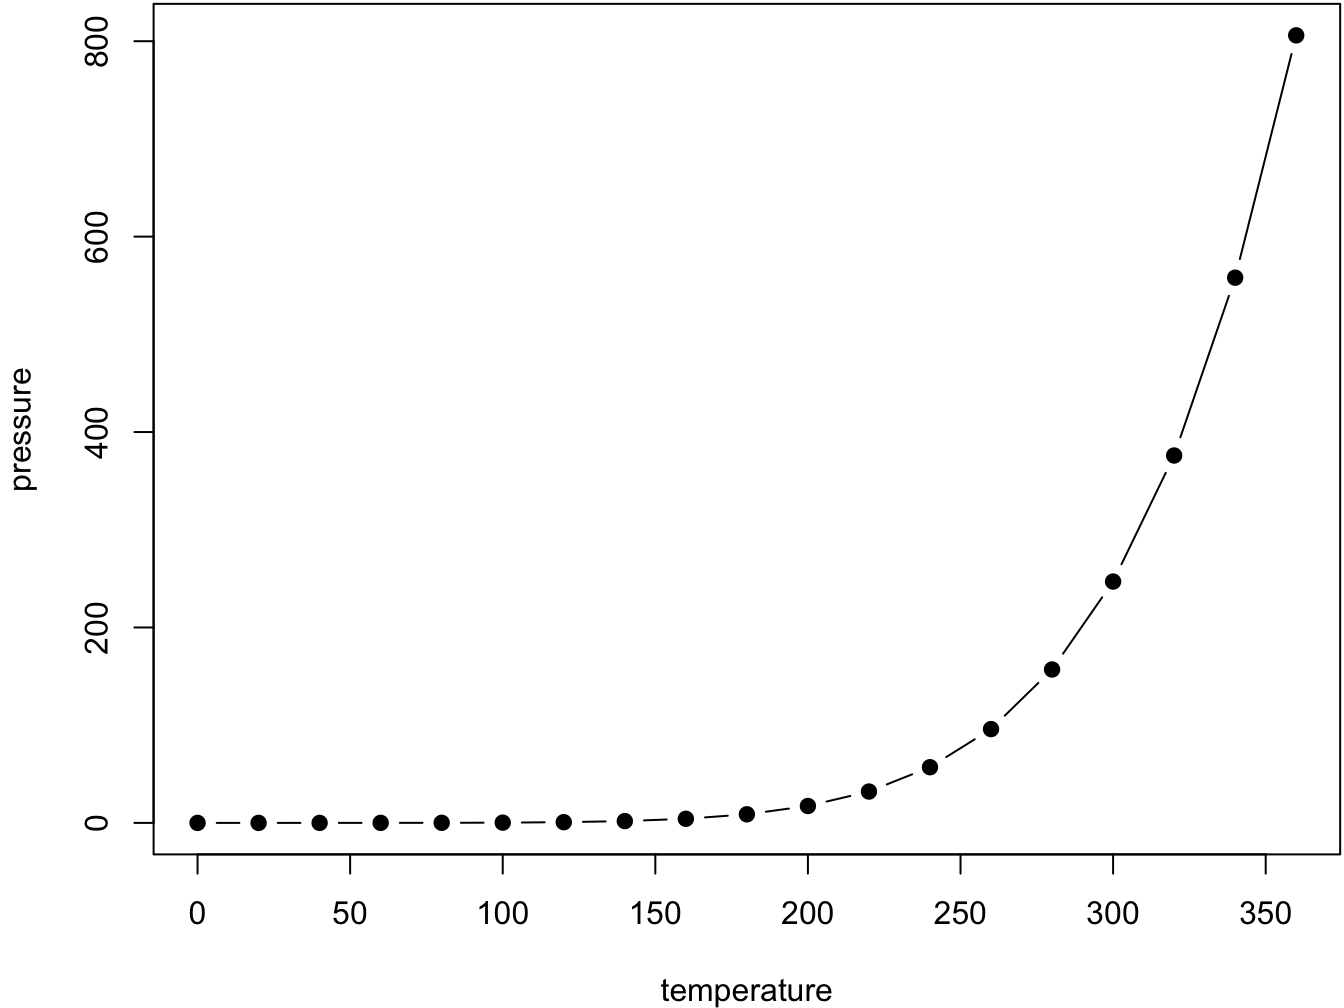
\includegraphics[width=0.8\linewidth]{prefresher_files/figure-latex/nice-fig-1} 

}

\caption{Here is a nice figure!}\label{fig:nice-fig}
\end{figure}

Reference a figure by its code chunk label with the \texttt{fig:}
prefix, e.g., see Figure \ref{fig:nice-fig}. Similarly, you can
reference tables generated from \texttt{knitr::kable()}, e.g., see Table
\ref{tab:nice-tab}.

\begin{Shaded}
\begin{Highlighting}[]
\NormalTok{knitr}\OperatorTok{::}\KeywordTok{kable}\NormalTok{(}
  \KeywordTok{head}\NormalTok{(iris, }\DecValTok{20}\NormalTok{), }\DataTypeTok{caption =} \StringTok{'Here is a nice table!'}\NormalTok{,}
  \DataTypeTok{booktabs =} \OtherTok{TRUE}
\NormalTok{)}
\end{Highlighting}
\end{Shaded}

\begin{table}

\caption{\label{tab:nice-tab}Here is a nice table!}
\centering
\begin{tabular}[t]{rrrrl}
\toprule
Sepal.Length & Sepal.Width & Petal.Length & Petal.Width & Species\\
\midrule
5.1 & 3.5 & 1.4 & 0.2 & setosa\\
4.9 & 3.0 & 1.4 & 0.2 & setosa\\
4.7 & 3.2 & 1.3 & 0.2 & setosa\\
4.6 & 3.1 & 1.5 & 0.2 & setosa\\
5.0 & 3.6 & 1.4 & 0.2 & setosa\\
\addlinespace
5.4 & 3.9 & 1.7 & 0.4 & setosa\\
4.6 & 3.4 & 1.4 & 0.3 & setosa\\
5.0 & 3.4 & 1.5 & 0.2 & setosa\\
4.4 & 2.9 & 1.4 & 0.2 & setosa\\
4.9 & 3.1 & 1.5 & 0.1 & setosa\\
\addlinespace
5.4 & 3.7 & 1.5 & 0.2 & setosa\\
4.8 & 3.4 & 1.6 & 0.2 & setosa\\
4.8 & 3.0 & 1.4 & 0.1 & setosa\\
4.3 & 3.0 & 1.1 & 0.1 & setosa\\
5.8 & 4.0 & 1.2 & 0.2 & setosa\\
\addlinespace
5.7 & 4.4 & 1.5 & 0.4 & setosa\\
5.4 & 3.9 & 1.3 & 0.4 & setosa\\
5.1 & 3.5 & 1.4 & 0.3 & setosa\\
5.7 & 3.8 & 1.7 & 0.3 & setosa\\
5.1 & 3.8 & 1.5 & 0.3 & setosa\\
\bottomrule
\end{tabular}
\end{table}

You can write citations, too. For example, we are using the
\textbf{bookdown} package \citep{R-bookdown} in this sample book, which
was built on top of R Markdown and \textbf{knitr} \citep{xie2015}.

\bibliography{book.bib,packages.bib}


\end{document}
